\documentclass[12pt,fleqn]{article}\usepackage{../../common}
\begin{document}
Log-Bariyer Yöntemi

Bir dışbükey probleme bakalım şimdi, artık tanıdık olan genel form bu,

$$
\min_x f(x) \quad \textrm{öyle ki}
$$
$$
h_i(x) \le 0, \quad i=1,..,m
$$
$$
Ax = b
$$

Tüm bu fonksiyonların dışbükey ve iki kere türevi alınabilir olduğunu farz
ediyoruz. Şimdi log bariyer metotu uygulayacağız, bu ilk göreceğimiz
iç-nokta yöntemi olacak [1, 14:00]. 

Bu yöntem ile önce eşitsizlik kısıtlamalarına tekabül eden bir log bariyer
fonksiyonu tanımlamak gerekiyor. Bu fonksiyon, 

$$
\phi(x) = -\sum_{i=1}^{m} \log(-h_i(x))
$$

Tabii $\log$'un negatif değerler üzerinde işletilemeyeceğini biliyoruz, o
sebeple üstteki eksi ile çarpım var (kısıtlamalara göre $h_i$'ler eksi
olmalı, onu da biliyoruz). Bu fonksiyon ile yapmaya uğraştığımız gösterge
(indicator) fonksiyonunu yaklaşıklamak. $\phi$'nin tanım kümesi $h$'ye göre
harfiyen olurlu olan $x$'ler. 

Şimdi log bariyerin yaklaşıklamayı nasıl yaptığına gelelim. Eşitlik
kısıtlamalarını atlarsak, üstteki minimizasyon problemi şu şekilde de
gösterilebilir [1, 15:53],

$$
\min_x f(x) + \sum_{i=1}^{m} I_{h_i(x) \le 0}(x)
$$

$I$ her $h_i$'nin sıfırdan küçük olup olmadığına göre 0 ya da çok büyük
değerler verir, bu yüzden üstteki gibi bir temsil, eşitsizlik
kısıtlamalarını kullanmakla eşdeğerdir. Çünkü minimizasyon problemi doğal
olarak çok büyük değerlerden kaçacak, ve böylece kısıtlamalar dolaylı
yoldan problem çözümüne dahil olmuş olacak. Altta kesikli çizgiyle
göstergeç fonksiyonu görülüyor, 

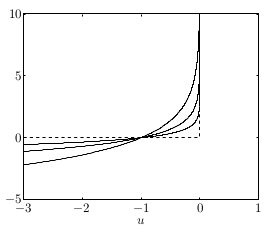
\includegraphics[width=15em]{func_59_barr_01.png}

Diğer kavisli çizgiler ise $-\log(-u) \frac{1}{t}$, her $t$ için farklı bir
eğri. $t$ büyütüldükçe log bariyer fonksiyonunu göstergeci daha da iyi
yaklaşık temsil etmeye başlıyor / ona yaklaşıyor [1, 17:08]. 

Altta farklı $\mu$ değerleri için
$-\mu \log(-u)$ fonksiyonun değerlerini görüyoruz. Fonksiyon görüldüğü gibi
$I$'ya oldukca yakın.

\begin{minted}[fontsize=\footnotesize]{python}
def I(u): 
   if u<0: return 0.
   else: return 10.0

u = np.linspace(-3,1,100)
Is = np.array([I(x) for x in u])

import pandas as pd
df = pd.DataFrame(index=u)

df['I'] = Is
df['$\mu$=0.5'] = -0.5*np.log(-u)
df['$\mu$=1.0'] = -1.0*np.log(-u)
df['$\mu$=2.0'] = -2.0*np.log(-u)

df.plot()
plt.savefig('func_59_barr_02.png')
\end{minted}

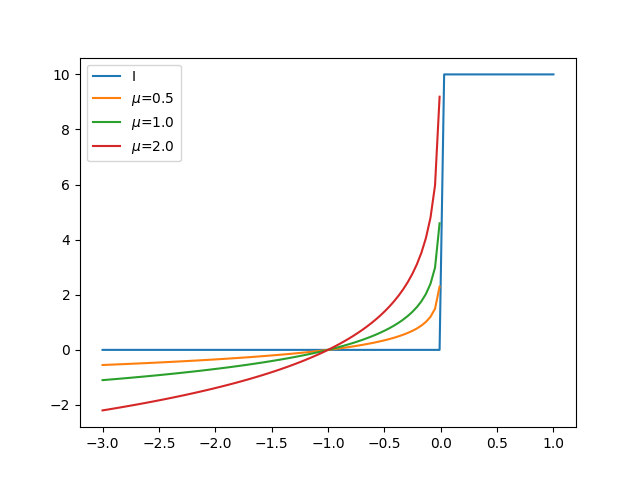
\includegraphics[width=25em]{func_59_barr_02.png}

Herhalde simdi en yapacagimiz tahmin edilebilir, gostergec fonksiyonlariyla
ile calismak zor, o zaman göstergeç toplamları log toplamları olarak
yaklaşıksallanabilir,

$$
\min_x f(x) + \frac{1}{t} \sum_{i=1}^{m} \log(-h_i(x))
$$

ki $t$ büyük olacak şekilde çünkü o zaman log, göstergeci iyi yaklaşık
olarak temsil ediyor, ardından bu yeni pürüzsüz problemi çözüyoruz,
eşitsizlik şartlarına ihtiyaç duymadan. 

Log-Bariyer Calculus

$\phi$ fonksiyonunun bazı özelliklerini dökmek faydalı olur, ileride Newton
metotundan bahsettiğimizde bu özellikler faydalı olacak. $\phi$ için gradyan ve
Hessian,

$$
\nabla \phi(x) = - \sum_{i=1}^{m} \frac{1}{h_i(x)} \nabla h_i(x)
$$

Hessian

$$
\nabla^2 \phi(x) = 
\sum_{i=1}^{m} \nabla h_i(x) \nabla h_i(x)^T - 
\sum_{i=1}^{m} \frac{1}{h_i(x)} \nabla^2 h_i(x)
$$

Merkezi gidiş yolu (central path)

Optimizasyon problemimizi $1/t$ yerine $t$ carpimi ile de gosterebiliriz,
yani

$$
\min_x t f(x) + \phi(x) \quad \textrm{öyle ki}
$$
$$
Ax = b
$$

Herneyse, merkezi yol $x^\ast(t)$, $t>0$'nin bir fonksiyonudur, yani her $t$
için eldeki çözümlerin ortaya çıkarttığı yoldur bir bakıma. Her $t$ için
problemin çözümünü KKT koşulları ile karakterize edebiliriz. 

$$
Ax^\ast(t) = b, \quad h_i(x^\ast(t)) < 0, \quad i=1,..,m
$$

$$
t \nabla f(x^\ast(t)) - \sum \frac{1}{h_i(x^\ast(t))} \nabla h_i(x^\ast(t)) + A^T w= 0
$$

Bu koşullar $x^\ast(t)$'nin optimal olmasının ne demek olduğunu
tanımlıyor. İki denklemdeki ilk denklem ana olurluktan geliyor, eşitlik
sınırlamalarına tekabül eden tek ikiz değişken var, $w$, onun işareti
üzerinde kısıtlama yok çünkü eşitlik kısıtlaması. Durağanlık koşulu ikinci
denklemde, ona nasıl eriştik? Problemin Lagrangian'i

$$
t f(x) + \phi(x) + w^T (Ax - b)
$$

Eğer $x$'e göre gradyan alıp sıfıra eşitlersek durağanlığı elde
ederim. Gradyan yeterli çünkü buradaki tüm fonksiyonlar dışbükey ve
pürüzsüz [1, 24:04]. 

Eğer üstteki problemi bir $w$ için çözersem o zaman merkezi yoldaki bir
çözümü belli bir $t$ için karakterize etmiş / tarif etmiş
oluyorum. Umudumuz o ki $t$'yi sonsuzluğa doğru büyüttükçe üstteki KKT
koşullarıyla temsil edilen çözümler orijinal problemimdeki çözüme
yaklaşmaya başlayacak. Bu olabilir değil mi? $t$'yi büyüttükçe log
bariyerin nasıl göstergeç fonksiyonuna benzemeye başladığını biraz önce
gördük. Bu tür log bariyerlerden oluşan optimizasyon problemi için de
benzer bir durum olacağını tahmin edebiliriz. 

Bu kavramları lineer programlar için yakından görebiliriz. Tüm bu
yaklaşımlar bu arada ilk başta LP'ler için ortaya atılmıştır. 

Önemli bir örnek,

$$
\min_x t c^T x - \sum_{i=1}^{m} \log(e_i - d_i^T x)
$$

Bu bir standart LP'nin bariyerleştirilmiş hali. Eşitlik kısıtlaması yok, ve
bariyer fonksiyonu çokyüzlü kısıtlama  $D x \le e$ ifadesine tekabül
ediyor. Bu problemi belli bir $t$ için çözersem, $t$'yi büyütürsem, bunu
ardı ardına tekrar edersem umudum orijinal LP'nin çözümüne yaklaşmak. 

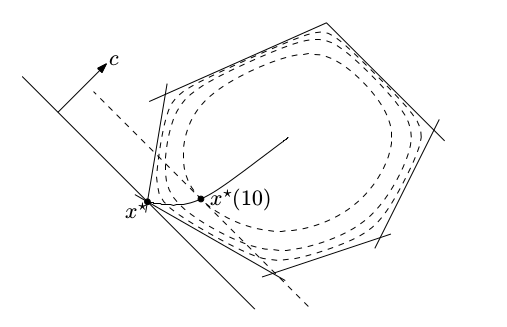
\includegraphics[width=20em]{func_59_barr_03.png}

Resimde görüldüğü gibi, ortadan başlıyoruz, $t=0$'da diyelim, ve $t$'yi
büyüttükçe yolda ilerliyoruz, ve sonuca erişiyoruz. Gidiş pürüzsüz, ve
LP'lerin karakterinden biliyoruz ki nihai sonuç çokyüzlümün (polyhedra)
ekstrem noktalarının birinde olmalı. Yarı yolda $t=10$'daki bir nokta
gösteriliyor, nihai sonuç belki $t=100$'da [2, 26:59]

KKT koşulu üzerinden durağanlığı temiz bir şekilde gösterebiliyoruz, ya da
iç nokta ve ortada, merkezde bir yol takip edilmesini zorlama bağlamında,
merkezlik şartı da deniyor buna, gradyan alınınca

$$
0 = tc - \sum_{i=1}^{m} \frac{1}{e_i - d_t ^T x^(t)} d_i
$$

Bu demektir ki gradyan $\nabla (x^\ast(t))$, $-c$'ye paralel olmalıdır, ya da
$\{ x: c^T x = c^T x^\ast(t) \}$ hiper düzlemi $\phi$'nin $x^\ast(t)$'deki
konturuna teğet durmalıdır [1, 28:12].

Ikiz noktalar

Birazdan merkezi yoldan ikiz noktalar alabileceğimizi göreceğiz. Bu çok
faydalı olacak çünkü bu ikiz noktaları bir ikiz boşluğu hesaplamak için
kullanacağız. Merkezi yoldayken bu yoldaki noktalar $x*(t)$'leri
kullanarak olurlu ikiz noktalar hesaplayabiliriz. Orijinal probleme
tekrar bakarsak, bu problem için ikiz değişkenleri elde etmek için her
eşitsizlik için bir $u_i$'ye, her eşitlik şartı için bir $v_i$'ya ihtiyacım
var. Onları nasıl tanımlarım? Merkezi yol üzerindeki çözümler üzerinden,

$$
u_i^\ast(t) = \frac{1}{t h_i(x^\ast(t))}, \quad i=1,..,m, \quad v^\ast(t) = w/t
$$

$w$ bariyer problemi için KKT koşullarını çözerken elde ettiğim değişken
idi. 

Niye üsttekiler orijinal problem için olurlu? Bunu görmek kolay, ilk önce,
$u_i^\ast(t)$'nin her ögesi harfiyen pozitif, çünkü $h_i(x^\ast(t))$'nin her
ögesi harfiyen negatif. Bu bariyer probleminin ana olurluk şartından
geliyor. Ayrıca $(u^\ast(t),v^\ast(t))$ Lagrange ikiz fonksiyonu $g(u,v)$'nin
tanım kümesinde (domain). Hatırlarsak Lagrange ikizi formülize ettiğimizde
tanım kümesinde bazı dolaylı sınırlamalar elde ediyorduk. Tarif itibariyle

$$
\nabla f(x^\ast(t)) + \sum_{i=1}^{m} u_i (x^\ast(t)) \nabla h_i(x^\ast(t)) + 
A^T v^\ast(t) = 0
$$


Yani $x^\ast(t)$, Lagrangian $L(x,u^\ast(t),v^\ast(t))$'i tüm $x$'ler üzerinden
minimize edeceği için $g(u^\ast(t),v^\ast(t)) > -\infty$. Bu direk durağanlık
şartından geliyor işte. O kadar bariz birşey ki aslında bazen kafa
karıştırıyor. Merkezi yol probleminden çözdüğümüz durağanlık koşulu
şöyleydi,

$$
t \nabla f(x^\ast(t)) - \sum \frac{1}{h_i(x^\ast(t))} \nabla h_i(x^\ast(t)) + A^T w= 0
$$

Bir $x^\ast$ çözümü ve $w$ olduğunu farz ediyoruz. Tüm formülü $t$ ile
bölersem,

$$
\nabla f(x^\ast(t)) - \sum \frac{1}{t h_i(x^\ast(t))} \nabla h_i(x^\ast(t)) + A^T \frac{w}{t}= 0
$$

Tek yaptığımız ``üstteki orijinal problemdeki durağanlık şartına çok
benziyor'' demek, değil mi, çünkü 

$$
\nabla f(x^\ast(t)) +
\sum \underbrace{\frac{-1}{t h_i(x^\ast(t))}}_{u_i} \nabla h_i(x^\ast(t)) + 
A^T \underbrace{\frac{w}{t}}_{v}= 0 
\mlabel{4}
$$

desem, orijinal problemin durağanlık şartına benzeyen bir ifade elde etmiş
olurum [2, 33:48]. Demiştik ki üstteki $u_i,v$ tanımları üzerinden orijinal
problem için olurlu ikiz noktaları alabiliyoruz. 

Soru: niye orijinal problem için optimal noktaları elde etmedim? Biraz önce
gördük, durağanlık koşulunu tatmin ettim, ana, ikiz olurluk
var.. ama.. tamamlayıcı gevşeklik tatmin edilmedi. Çok önemli. Onun yerine
ne var? $u_i h_i (x) = 0$ olması lazım, onun yerine ne var? Tanım
itibariyle $u_i = -1/t ..$ var. O zaman sıfıra yakınsak çok yakınsak bölüm
büyür, dolaylı olarak $t$'yi büyüttükçe orijial problemin KKT koşullarını
yaklaşıksallamış oluruz. O zaman log bariyer problemini çözmüş olmamıza
rağmen belli bir $t$ değer için orijinal problem için çözüm olmamasının
sebebi tamamlayıcı gevşekliğin tatmin edilmiyor olması.

Ama elimizdekiler hala çok faydalı, çünkü herhangi bir anda merkez yol
üzerinde $t$'nin fonksiyonu olarak ne kadar alt optimal olduğumuzu
sınırlamak mümkün oluyor. Bunun için sadece ikiz boşluğunu hesaplıyoruz, o
kadar. O zaman $u^\ast,v^\ast$'da Lagrange ikiz fonksiyonu hesaplıyorum, ve $f^\ast$
ile bu Lagrange farkını buluyorum, ve ikiz boşluğu hesaplanmış oluyor. 
(4)'te gördük ki $x^\ast$ Lagrangian'i $u^\ast,v^\ast$'da minimize eder, o zaman
ikizi alttaki gibi hesaplayarak 

$$
g(u^\ast(t),v^\ast(t)) = 
f(x^\ast(t)) + \sum_{i=1}^{m} u_i^\ast(t) h_i(x^\ast(t)) + v^\ast(t)^T (Ax^\ast(t) - b)
$$

Büyük toplamdaki ikinci terim sıfır, çünkü merkezi yolda $Ax^\ast$ her zaman
$b$'ye eşittir. Birince terimde, $u_i$'i $-1/t$'ye eşitledik, ve bu $m$
kere toplanacak, sonuç

$$
= f(x^\ast(t)) - m/t
$$

Yani göstermiş olduk ki merkezi yolun optimallikten olan uzaklığı en fazla
$m/t$ olacaktır,

$$
f(x^\ast(t)) - f^\ast \le m/t
$$

Üstteki bariyer metorun işlediğine dair ispata en yakın sonuç, bize diyor
ki eğer herhangi bir $t$ için bariyer problemini çözersem optimalliğe
yakınlık her zaman $m/t$'den küçük olur. $t$'yi isteğe bağlı olarak
büyüttükçe o ölçüde optimalliğe yaklaşmış olurum. 

Merkezi yolu yorumlamanın bir diğer yolu ``sarsıma uğratılmış KKT
koşulları'' denen bir teknik üzerinden. Şimdiye kadar gördük ki merkez yol
ve ona tekabül eden ikiz değerler (4)'teki durağanlık şartını çözüyor. 
$u_i \ge 0$, $h_i(x) \le 0$, ve $Ax = b$. Tamamlayıcı gevşeklik haricinde tüm
koşullar tatmin. Esas KKT koşullarında 

$$
u_i^\ast(t) \cdot h_i^\ast(t) = 0, \quad i=1,..,m
$$

olurdu, biz onun yerine 

$$
u_i^\ast(t) \cdot h_i^\ast(t) = -1/t, \quad i=1,..,m
$$

dedik. Yani bir anlamda log bariyer fonksiyonunu unutuyoruz, onun yerine şu
probleme bakıyoruz,

$$
\nabla f(x^\ast(t)) + \sum_{i=1}^{m} u_i(x^\ast(t))\nabla h_i(x^\ast(t)) + A^T v^\ast(t) = 0
$$

$$
u_i^\ast(t) \cdot h_i^\ast(t) = -1/t, \quad i=1,..,m
$$

$$
h_i(x^\ast(t)) \le 0, \quad i=1,..,m, \quad Ax^\ast(t) = b
$$

$$
u_i(x^\ast(t)) \ge 0
$$

Ve $t$'yi büyüterek üstteki problemi çözüyorum. Yani olurluğu, durağanlığı
tam olarak, tamamlayıcı gevşekliği ise yaklaşık olarak çözmüş oluyorum, ve
yaklaşıksallığı gittikçe büyüyen $t$'ler üzerinden daha sıkı hale getiriyorum. 
Yani log bariyer tekniği ile sarsıma uğratılmış KKT koşulları sınırlı
problemleri çözmenin iki yolu. 

Niye ufak $t$ ile başlayıp büyütüyorum [2, 02:19]? Çünkü pratikte bu iyi
işliyor. Niye işlediğini görmek zor değil, $t$ küçükken tüm fonksiyon
oldukca pürüzsüz, ve onun üzerinde Newton adımları rahat işler. Ama $t$'yi
büyüttükçe onun kontrol ettiği fonksiyon kısımlarını gittikçe daha az
pürüzsüz yapmaya başlıyorum, ama bu çok kötü değil çünkü bu noktada çözüm
bölgesine kabaca yaklaşmış olmalıyım. 

Yakınsama analizi (convergence analysis) 

Teori 

Diyelim ki merkezleştirme adımlarını kesin olarak çözebiliyoruz, yani,
diyelim ki ne zaman Newton metotunu uygularsam mükemmel bir sonuç
alıyorum. Tabii ki bu gerçekte olmuyor ama farz edelim. O zaman, sadece
$t$'yi her adımda $\mu$ ile çarpmamızın doğal sonucu olarak ve ikizlik
boşluğununun $m / t$ olması sebebiyle $k$ adım sonrası alttakini görürdük, 

$$
f(x^(k)) - f^\ast \le \frac{m}{\mu^k t^{0}}
$$

Bu ifade diyor ki istenen $\epsilon$ seviyesinde bir doğruluğa erişmek için 

$$
\frac{\log ( m / (t^{(0)} \epsilon) )}{\log \mu}
$$

tane merkezleştirme adımına ihtiyacımız var. 

Olurluk metotu (feasibility method)

Bariyer metotunun bir noktadan başlaması gerekir ve bu nokta olurlu
olmalıdır. Olurlu derken 

$$
h_i(x) < 0, \quad i=1,..,m, \quad Ax = b
$$

şartlarına uyan bir noktadan bahsediyorum. Fakat ya öyle bir nokta elimizde
yoksa? Başta olurlu olan bir noktayı bulmanın kendisi de zor bir
problem. Böyle bir noktayı elde etmek için olurluk metotu denen bir yöntem
kullanmak gerekecek. Boyd'un kitabı [4, Bölüm 11] bu metota ``1. Faz (Phase
I)'' ismi veriyor, problemin kendisini çözmeye ``2. Faz'' diyor. Pratikte
bariyer metotunu kullanmak isteyenler bunu hatırlamalı.

Harfiyen olurlu bir noktayı nasıl buluruz? Kulağa biraz dolambaçlı gibi
gelebilir ama bu noktayı bulmak için ayrı, farklı bir optimizasyon problemi
daha kurarız, onu da bariyer metotu ile çözeriz. Tabii illa bariyer metotu
olması gerekmez, ana-çift iç-nokta yöntemi de olabilir, ama her halükarda
alttaki problemi çözeriz. 

Bu problemde elimizde iki tane değişken grubu var, $x,s$. Problem [2, 23:02], 

$$
\min_{x,s} s \quad \textrm{öyle ki}
$$
$$
h_i(x) \le s, \quad i=1,..,m
$$
$$
Ax = b
$$

Amaç harfiyen negatif bir $s$ elde etmek, böylece $h_i(x) \le s$ üzerinden
ana problemin eşitsizlik şartları tatmin olacak, ayrıca $Ax = b$'e uygun
bir başlangıç noktası elde edilmiş olacak ki bu da ana problem için
gerekli. 

Bu problemi bariyer metotu ile çözmek oldukca kolay, ana problemin kendisi
kadar zor değil. Niye? İki sebep: ilki, üstteki problemi çözmek için de
harfiyen olurlu bir başlangı noktası lazım, ama bu noktayı bulmak aslında
çok kolay. Bana tek gereken eşitlik kısıtlaması $Ax = b$'yi tatmin eden bir
$x$ bulmak, ama bu lineer bir sistem çözümü, her lineer cebir paketi bunu
çözer. Ardından elde edilen $x$ ile $h_i(x)$'i hesaplamak, ve bunların en
büyüğünü artı mesela 0.01 diyerek kullanmak [2, 24:00]. Elde edeceğimiz
sonuç üstteki problem için harfiyen olurludur, eşitsizlik kısıtlamalarına
harfiyen uygun. Şimdi elimde bir başlangıç $x$'i ve $s$'i var, ve buradan
başlayarak bariyer metotunun adımlarını uygulayabilirim. İşin güzel tarafı
durma şartımız çok basit, $s$'in her ögesinin negatif olduğunu gördüğüm
anda şak diye durabilirim, yani üstteki programın ``optimal'' olmasıyla
ilgilenmiyorum sonuçta bana tek gereken ana problemim için olurlu bir
başlangıç noktası. Çoğunlukla yapılan tarif edilen şekilde $x,s$ bulmak ve
bunu ardı ardına yapmak ta ki tamamen negatif elde edilene kadar ve o
noktada durulur, ana probleme dönülür.

Alternatif olarak şu problem de çözülebilir,

$$
\min_{x,s} 1^T s, \quad \textrm{öyle ki}
$$
$$
h_i(x) \le s_i, \quad i=1,..,m
$$
$$
Ax = b, s \ge 0
$$

Bu metotun avantajı eğer sistem olurlu değilse hangi kısıtlamanın harfiyen
yerine getirilemediğini bize söyler. Dezavantaj çözmesinin biraz daha zor
olabilmesi.

Ekler

Bir diğer başlangıç noktası bulma metotu, Faz I yaklaşımı daha [5]. Burada

$$
\min t, \quad \textrm{öyle ki}
$$
$$
Ax = b, \quad x \ge (1-t) 1, \quad t \ge 0
$$

problemini çözüyoruz, ki değişkenler $x$ ve $t \in \mathbb{R}$. Eğer
üstteki problemde $t < 1$ olacak şekilde olurlu bir $x,t$ bulabilirsek, o
zaman elimizdeki $x$ orijinal problem için de harfiyen olurlu
olacaktır. Argümanın tersi de geçerli, esas LP harfiyen olurludur sadece ve
sadece $t^\ast < 1$ ise ki $t^\ast$ Faz I probleminin optimal değeri.

Ama şimdi üstteki problem için nasıl başlangıç değeri buluruz sorusu var,
ama bu daha basit. $Ax^0 = b$'ye çözüm olan herhangi bir $x^0$'yu alırız,
ve $t^0 = 2 - \min_i x_i^0$ seçeriz. Tabii eğer $\min_i x_i^0 < 0$ değil
ise, yani tüm $x_i$'lar pozitif ise, o zaman iş bitti demektir, $x^0$ zaten
harfiyen olurlu. Değil ise log bariyer ile devam edeceğiz, problemi
standart forma çevirmek için $z = x + (t-1)\vec{1}$ diyebiliriz,

$$
z = x + t \vec{1} - \vec{1}
$$

Ya da

$$
x = z - t\vec{1} + \vec{1}
$$

Bunu $Ax = b$ üzerinde uygularsak, 

$$
A (z - t\vec{1} + \vec{1}) = b
$$

$$
Az - A t\vec{1} = b - A\vec{1}
$$

Eşitliğin solundakiler yerine $x$'i genişletip $t$ için yeni bir hücre
yaratabiliriz, ve $A$'ya yeni kolon ekleriz, bu kolondaki her öge mevcut
$A$'nin satırlarının toplamının negatifi olur. Bedel vektörü de
$c = [0, 0, ..., 1]$ haline gelir, son öğe $t$ için.

Standard LP çözen bariyer metot temelli [3] kod alttadır. 

\inputminted[fontsize=\footnotesize]{python}{barr.py}

Örnek olarak uyduruk bir problem seçtik, problem özellikle başta olurlu
nokta bulamayacak şekilde ayarlandı, böylece gidip kendimizin bulması
gerekiyor.

\begin{minted}[fontsize=\footnotesize]{python}
import numpy as np
from scipy.optimize import linprog
import barr

import barr

A = [[1.,  1., 1., 0.],
     [1.,  3., 0., 1.],
     [9.,  1., -3., 1.]]
b = [[5., 7., -1]]
c = [[-1., -5., 0., 0. ]]

A = np.array(A)
b = np.array(b).T
c = np.array(c).T

x_star,gap,nsteps = barr.lp_solve(A,b,c)

print ('log bariyer ==========')
print (x_star)

res = linprog(c, A_eq=A, b_eq=b)
print ('linprog ===============')
print (res)
\end{minted}

\begin{verbatim}
phase I
[[1.44060995]
 [3.1918138 ]
 [3.37720706]
 [1.        ]
 [2.00321027]]
log bariyer ==========
[4.37502314e-01 2.18747454e+00 2.37502314e+00 7.40628401e-05]
linprog ===============
     con: array([ 2.05213624e-11,  2.05719886e-11, -9.18283227e-11])
     fun: -11.37499999994356
 message: 'Optimization terminated successfully.'
     nit: 4
   slack: array([], dtype=float64)
  status: 0
 success: True
       x: array([4.3750000e-01, 2.1875000e+00, 2.3750000e+00, 1.0991855e-11])
\end{verbatim}

Şimdi daha önce de çözdüğümüz bir örneğe tekrar bakalım,

$$
\min_x -x_1 - 5x_2 \quad \textrm{öyle ki}
$$
$$
x_1 + x_2 + x_3  = 5 
$$
$$
x_1 + 3 x_2 + x_4 = 7
$$
$$
x_1,x_2,x_3,x_4 \ge 0
$$

\begin{minted}[fontsize=\footnotesize]{python}
A = np.array([[1,  1, 1, 0],
              [1,  3, 0, 1]])
b = np.array([5,7])
c = np.array([-1, -5, 0, 0 ])
A = np.array(A)
b = np.array(b).T
c = np.array(c).T

x_star,gap,nsteps = barr.lp_solve(A,b,c)

print ('log bariyer ==========')
print (x_star)

res = linprog(c, A_eq=A, b_eq=b)
print ('linprog ===============')
print (res)
\end{minted}

\begin{verbatim}
Ax=b solution already feasible
log bariyer ==========
[1.87451194e-04 2.33324585e+00 2.66656670e+00 7.49883368e-05]
linprog ===============
     con: array([1.18571819e-11, 1.18527410e-11])
     fun: -11.66666666664022
 message: 'Optimization terminated successfully.'
     nit: 4
   slack: array([], dtype=float64)
  status: 0
 success: True
       x: array([1.15454732e-13, 2.33333333e+00, 2.66666667e+00, 3.96953400e-12])
\end{verbatim}

Bu durumda $Ax^0=b$ çözümü başlangıç için yeterliydi ve o kullanıldı.

Gradyan ve Hessian

Pek çok yerde kullanılan bir eşitsizlik görelim, mesela bütün $x_i < 0$
olduğu bir durum, yani $h_i(x) = -x$. O zaman bariyer neye benzer? 

$$
\phi(x) = - \sum_{i=1}^{n} \log x_i
$$

$$
\nabla \phi(x) = - \left[\begin{array}{c}
1/x_1  \\ 
\vdots \\
1/x_n
\end{array}\right] 
= - X^{-1} \vec{1}
$$

Burada $X$ matrisi 

$$
X = \diag(x) = 
\left[\begin{array}{ccc}
x_1 & & \\
    & \ddots & \\
    & & x_n
\end{array}\right]
$$

ve $\vec{1}$ sembolu tamamen 1'lerden oluşan matris. 

Hessian

$$
\nabla^2 \phi (x) = \left[\begin{array}{ccc}
1/x_1^2 & & \\
    & \ddots & \\
    & & 1/x_n^2
\end{array}\right] = X^2 
$$

Eski Anlatım

$$
\min_x f(x),  \quad  \textrm{öyle ki}, 
$$
$$
c_i(x) \ge 0, \quad i=1,2,..,m
$$

$c_i$ ile gösterilen eşitsizlik içeren (üstte büyüklük türünden)
kısıtlamalar olduğunu düşünelim. Bu problemi nasıl çözeriz?

Bir fikir, problemin eşitizliklerini bir gösterge (indicator)
fonksiyonu üzerinden, Lagrange yönteminde olduğu gibi, ana hedef
fonksiyonuna dahil etmek, ve elde edilen yeni hedefi kısıtlanmamış bir
problem gibi çözmek. Yani üstteki yerine, alttaki problemi çözmek,

$$
\min_x f(x) + \sum_{i=1}^{m} I(c_i(x))
$$

ki $I$ pozitif reel fonksiyonlar için göstergeç fonksiyonu,

$$
I(u) = 
\left\{ \begin{array}{ll}
0 & u \le 0 \\
\infty & u > 0
\end{array} \right.
$$

Bu yaklaşımın nasıl işleyeceğini kabaca tahmin edebiliriz. $I$ fonksiyonu
0'dan büyük değerler için müthiş büyük değerler veriyor, bu sebeple
optimizasyon sırasında o değerlerden tabii ki kaçınılacak, ve arayış
istediğimiz noktalara doğru kayacak. Tabii $x_1 > 3$ gibi bir şart varsa
onu $x_1 - 3 > 0$ şartına değiştiriyoruz ki üstteki göstergeci
kullanabilelim. Bu yaklaşıma "bariyer metotu" ismi veriliyor çünkü $I$ ile
bir bariyer yaratılmış oluyor.

Fakat bir problem var, göstergeç fonksiyonunun türevini almak, ve pürüzsüz
rahat kullanılabilen bir yeni fonksiyon elde etmek kolay değil. Acaba $I$
yerine onu yaklaşık temsil edebilen bir başka sürekli fonksiyon kullanamaz
mıyız?

Log fonksiyonunu kullanabiliriz. 
O zaman eldeki tüm $c_i(x) \ge 0$ kısıtlamalarını

$$
- \sum_{i=1}^{m} \log c_i(x)
$$

ile hedef fonksiyonuna dahil edebiliriz, yeni birleşik fonksiyon,

$$
P(x;\mu) = f(x) - \mu \sum_{i=1}^{m} \log c_i(x) 
$$

olur. Böylece elde edilen yaklaşım log-bariyer yaklaşımı
olacaktır. Mınımizasyon sırasında hem başta bariyerden kaçınilmiş olunacak,
hem de $\mu$ küçükdükçe hedefin geri kalanında istenilen minimal değerlere
doğru kayılmış olunacak. 

Algoritma olarak optimizasyon şu şekilde gider;

1) Bir $x$ ve $\mu$ değerinden başla.

2) Newton metotu ile birkaç adım at (durma kriteri yaklaşıma göre değisebilir)

3) $\mu$'yu küçült

4) Ana durma kriterine bak, tamamsa dur. Yoksa başa dön

Bu yaklaşımın dışbükey (convex) problemler için global minimuma
gittiği ispatlanmıştır [4, sf. 504].

Örnek

$\min (x_1 + 0.5)^2 + (x_2 - 0.5)^2$ problemini çöz, $x_1 \in [0,1]$ ve $x_2 \in
[0,1]$ kriterine göre.

Üstteki fonksiyon için log-bariyer,

$$
P(x;\mu) = (x_1 + 0.5)^2 + (x_2-0.5)^2 -
\mu 
\big[
\log x_1 + \log (1-x_1) + \log x_2 + \log (1-x_2)
\big]
$$

Bu formülasyonu nasıl elde ettiğimiz bariz herhalde, $x_1 \ge 0$ ve
$x_1 \le 1$ kısıtlamaları var mesela, ikinci ifadeyi büyüktür
işaretine çevirmek için eksi ile çarptık, $-x_1 \ge 1$, ya da $1-x_1
\ge 0$ böylece $\log(1-x_1)$ oldu.

Artık Newton yöntemini kullanarak sanki elimizde bir kısıtlanması
olmayan fonksiyon varmış gibi kodlama yapabiliriz, $P$'yi minimize
edebiliriz. Newton yönü $d$ için gereken Hessian ve Jacobian
matrislerini otomatik türevle hesaplayacağız, belli bir noktadan
başlayacağız, ve her adımda $d = -H(x)^{-1} \nabla f(x)$ yönünde adım
atacağız.

\begin{minted}[fontsize=\footnotesize]{python}
from autograd import numpy as anp, grad, hessian, jacobian
import numpy.linalg as lin

x = np.array([0.8,0.2])
mu = 2.0
for i in range(10):
    def P(x):
    	x1,x2=x[0],x[1]
    	return (x1+0.5)**2 + (x2-0.5)**2 - mu * \
	   (anp.log(x1) + anp.log(1-x1) + anp.log(x2)+anp.log(1-x2))

    h = hessian(P)
    j = jacobian(P)
    J = j(np.array(x))
    H = h(np.array(x))
    d = np.dot(-lin.inv(H), J)
    x = x + d
    print (i, x, np.round(mu,5))
    mu = mu*0.1
\end{minted}

\begin{verbatim}
0 [0.61678005 0.34693878] 2.0
1 [-0.00858974  0.486471  ] 0.2
2 [-0.02078755  0.49999853] 0.02
3 [-0.18014768  0.5       ] 0.002
4 [-0.49963245  0.5       ] 0.0002
5 [-0.50002667  0.5       ] 2e-05
6 [-0.50000267  0.5       ] 0.0
7 [-0.50000027  0.5       ] 0.0
8 [-0.50000003  0.5       ] 0.0
9 [-0.5  0.5] 0.0
\end{verbatim}

Görüldüğü gibi 5. adımda optimal noktaya gelindi, o noktada $\mu$
oldukca küçük, ve bariyerle tanımladığımız yerlerden uzak duruldu,
optimal nokta $x_1=-0.5,x_2=0.5$ bulundu.


Kaynaklar

[1] Tibshirani, 
    {\em Convex Optimization, Lecture Video 15, Part 1}, 
    \url{https://www.youtube.com/channel/UCIvaLZcfz3ikJ1cD-zMpIXg}   

[2] Tibshirani, 
    {\em Convex Optimization, Lecture Video 15, Part 2}, 
    \url{https://www.youtube.com/channel/UCIvaLZcfz3ikJ1cD-zMpIXg}   

[3] Bao, {\em LP-Solver, Github}, 
    \url{https://github.com/rayjim/python_proj/blob/master/hm_8/lp_solver.py}

[4] Boyd, {\em Convex Optimization}

[5] Boyd, {\em Convex Optimization, Solutions to additional exercises}

\end{document}



